\subsection{Passivity Analysis}

The kinetic energy of the system is given as:
\begin{equation}
	W(\vecs \xi, \vecs{\dot \xi}) = \frac{1}{2}  \dot{\vecs{\xi}}^T \matd{M}(\vecs \xi) \dot{\vecs{\xi}} \label{eq:energy_system}
\end{equation}

% \begin{theorem} \label{theorem:passivity}
%   Let $\vect f(\xi)$ is are desired dynamics with bounded magnitude, i.e., $\| \vect f(\xi) \| < v^{\mathrm{max}}, \forall \xi \in \mathbb{R}^N$.
%   Let the system \eqref{eq:robot_dynamics} be controlled by \eqref{eq:control_command} using is \eqref{eq:damping_summation}.
%   There exists a (lower) limit velocity $\vecs{\bar v} = \text{const.}$ such that the system is passive with respect to the input-output pair $\vecs \xi_e$, $\vecs{\dot \xi}$ when exceeding the limit velocity, i.e., $\dot{W} \leq \vecs{\dot \xi}^T \vecs \tau_e, \; \forall \vecs \xi \in \mathbb{R}^N: \| \vecs{\dot \xi} \| \geq \vecs{\bar v}$ and the storage function being the kinetic energy $W \in \mathbb{R}$ given in \eqref{eq:energy_system}
% \end{theorem}
  
\begin{proof}
The time derivative of storage function $W$ can be evaluated as:
\begin{align}
  % \begin{split}
    \dot W(\vecs \xi, \vecs{\dot \xi}) &=
    \vecs{\dot \xi}^T \matd M(\vecs \xi) \vecs{\ddot \xi}  + \frac{1}{2} \vecs{\dot \xi}^T \dot{\matd M}(\vecs \xi) \vecs{\dot \xi}  \nonumber \\
  &= \frac{1}{2} \vecs{\dot \xi}^T \left( \dot{\matd M}(\vecs \xi) - 2 \matd C(\vecs \xi) \right) \dot{\vecs \xi} - \vecs{\dot \xi}^T \matd{D}(\vecs \xi) \vecs{\dot \xi} + \vecs{\dot \xi}^T \vecs \tau_e \nonumber \\
  &= - \vecs{\dot \xi}^T \matd{D}(\vecs \xi) \left( \vecs{\dot\xi} - \mathbf{f}(\vecs \xi) \right) + \vecs{\dot\xi}^T \tau_e
  % \end{split}
\end{align}
where we use the fact that $\dot{\matd M} - 2 \matd C$ is skew symmetric, and hence the corresponding sumand is zero.

Note, that even if we use a coriolis compensation in the control law, the corresponding term does not vanish. However, the mass matrix $\matr M(\vecs \xi)$ is a system property and it has an upper limit. Hence, this upper limit can be thought of as the maximum the storage function.

\subsubsection{Stability with Uniform Damping}
Let us investigate the region where the passivity holds. For this, we first look at the simplest case where all damping values are equal to one. Hence we have:
\begin{equation}
	\matd{D}({\vecs \xi}) = \matd{Q}({\vecs \xi}) \matd{S} ({\vecs \xi}) \matd{Q}({\vecs \xi})^{-1}= \matd{Q}({\vecs \xi}) \matd{I} \matd{Q}({\vecs \xi})^{-1} = \matd{I}
\end{equation}
where $\matd{I}$ is the identity matrix.

It follows that the system is passive with respect to the input, the external force $\tau_e$, and the output, the velocity $\dot {\vecs \xi}$, as long as:
\begin{equation}
	\dot{\boldsymbol {\vecs \xi}}^T \matd{D}({\vecs \xi}) \left(\dot{\boldsymbol {\vecs \xi}} - \boldsymbol{f}(\boldsymbol {\vecs \xi}) \right) = 
    \dot{{\vecs \xi}} ^ T \Delta \vect{f}  \geq 0 
 \; , \quad
 \Delta \mathbf{f} = \dot{{\vecs \xi}} - \mathbf{f}({\vecs \xi})
\end{equation}

On the border of this region, the two vectors $\Delta \mathbf{f}$ and $\dot{\mathbf {\vecs \xi}}$ are orthogonal.
Hence using Thale's theorem, this region can be evaluated as a circle with radius $\| \mathbf{f} ({\vecs \xi}) \| / 2$ and center $\mathbf{f}(\mathbf {\vecs \xi}) / 2$, as visualized in Figure~\ref{fig:passivity_analysis}.

\begin{figure}[b]
	\centering
	% \includesvg[width=0.7\columnwidth]{figures/passivity_analysis.svg}
    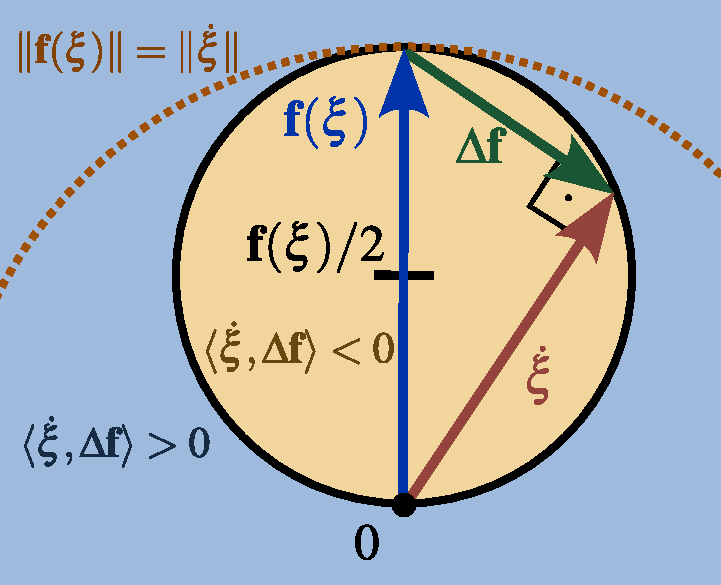
\includegraphics[width=0.7\columnwidth]{figures/passivity_analysis}
	\caption{In the velocity space, the region of non-passivity is circular (red). All remaining desired velocity $\mathrm f(\mathrm{{\vecs \xi}})$ and observed velocity $\dot{\mathrm {\vecs \xi}}$ pairs ensure passivity (green region).}
	\label{fig:passivity_analysis}
\end{figure}

% \subsubsection{Global Stability}
Moreover, the system is passive as long as the observed velocity $\dot{{\vecs \xi}}$ is outside the circular-red region, which is a subset of the region where the magnitude of the observed velocity is smaller than the desired velocity $\mathbf{f}({\vecs \xi})$, i.e.,
\begin{equation}
	\dot W({\vecs \xi}, \dot{{\vecs \xi}}) \leq \dot{{\vecs \xi}}^T \vecs \tau_e
 \quad \forall {\vecs \xi} : \| \dot{{\vecs \xi}} \| \geq\| \mathbf{f}({\vecs \xi}) \| 
\end{equation}
% \footnote{Note that the region of passivity is even larger, but we this region is sufficient for our purposes. As it indicates that there is only non-passivity of the system to speed when the current velocity is too slow.}

As in the red region, the system is not passive, the storage function $W$ could increase, and hence the velocity $\dot {\vecs \xi}$ could increase in a non-passive manner. However, the velocity increase is limited to staying below $\| \vect f({\vecs \xi}) \|$ before the system enters a passive state. Moreover, for the case in which we approach a stable region $\boldsymbol{f}({\vecs \xi}) \rightarrow \vect{0}$, the system becomes passive for any velocity $\boldsymbol{\vecs{\dot \xi}}$.

This behavior is not unexpected, as the controller is designed to approach a desired DS $\vect{f}({\vecs \xi})$. Hence, as long as the desired velocity is not reached, the kinetic energy increases even with no force input $\vecs \tau_e$.

It follows that the system is stable as long as the desired velocity $\mathbf{f}({\vecs \xi})$ is stable and the input $\int_{0}^T \dot{{\vecs \xi}}^T \vecs \tau_e dt$ is bounded. Since as soon as the observed velocity $\| \dot{{\vecs \xi}} \| $ is larger than the desired velocity, the system behaves passively. Hence, the control cannot introduce unexpected energy.

\subsubsection{Stability with General Damping}
The damping matrix $\matd{D}({\vecs \xi}) = \matd{Q}({\vecs \xi}) \matd{S}({\vecs \xi}) \matd{Q}({\vecs \xi})^{-1}$, can be interpreted as a coordinate transfer, such that:
\begin{equation}
	\vecs{\bar v} = \sqrt{\matd{S}({\vecs \xi})} \matd{Q}({\vecs \xi})^{-1} \dot{{\vecs \xi}}
	\quad \text{and} \quad
	\bar{\Delta \mathbf f} = \sqrt{\matd{S}({\vecs \xi})} \matd{Q}({\vecs \xi})^{-1} \Delta \mathbf{f}
\end{equation}
where the square root of the diagonal matrix $\Lambda({\vecs \xi})$ is taken element-wise. Thus, we get:
\begin{equation}
\dot{\vecs \xi}^T \matd{D}({\vecs \xi}) \Delta \mathbf{f} = \vecs{\dot \xi}^T \matd{Q}({\vecs \xi}) \matd{S}({\vecs \xi}) \matd{Q}({\vecs \xi})^{-1} \Delta \mathbf{f} = \vecs{\bar v}^T \bar{\Delta \mathbf f}
\end{equation}
The analysis described in Fig.~\ref{fig:passivity_analysis} can hence be applied in the transformed space, too. 

For an orthogonal decomposition matrix $\matd{Q}(\boldsymbol{{\vecs \xi}})$, the region of non-passivity is an ellipse with axes equal to the columns of $\matd{Q}({\vecs \xi})$, and the corresponding axes lengths are the diagonal elements of $\| \mathbf{f}({\vecs \xi})^T \sqrt{\matd{S}({\vecs \xi})}\| / 2 \sqrt{\matd{S}({\vecs \xi})}^{(-1)}$. 

If the axes' lengths are large, this can lead to accelerating the velocity even though it is already larger (but not pointing in the correct direction) than the desired velocity. However, the region is still clearly bounded by the ellipse.

Similarly, this extends to a basis $\matd{Q}$, which is not orthogonal. However, in such a case, the controller must be carefully chosen to ensure that the speed up is limited when the basis is close to singular (i.e., by limiting the relative difference of the stretching vectors).

The results apply to a general shape of a damping matrix $\matd{D}$. This implies that global stability for an underlying stable system extends to the general passive interaction control introduced in \cite{kronander2015passive}.
\end{proof}

Note that while the passivity statement is local only, the system might exit the passive region. However, passivity is used to prove that a controller does not \textit{pump} energy into a system. In the present case, we have an upper limit on the velocity (and hence the kinetic energy), where the system is shown to be passive. Hence, even if the controller increases the system's energy above this limit, it becomes passive again. Hence, the controller is ensured not to increase the system's energy.

% \subsection{Obstacle Aware Eigenvalues}
% Let us define nominal eigenvalues as $\lambda$, the DS-following values as $\lambda^{DS}$ and the obstacle-avoiding ones as $\lambda^{\mathrm{max}}$, for a given distance weight $w$, the eigenvalues in normal direction are defined as
% \begin{equation}
%     \lambda_n = (1 - w) \lambda + w \lambda^{\mathrm{max}}
% \end{equation}

% In order to obtain these values in the direction, the eigenvalues along the first eigenvalue (the direction of the ds) are evaluated as follows:
% \begin{equation}
% \begin{split}
%  \lambda_1 = \max \left( w_1 \lambda^{\mathrm{max}} + ( 1 - w_1) \lambda^{DS}, \lambda^{DS}\right) \\
%  \quad \text{with} \quad
%  w_1 = \max \left( \sqrt{2} / 2 | \langle e_1 , e_n \rangle |, 1 \right)
% \end{split}
% \end{equation}

% Furthermore, the eigenvalues along the second direction can be set as:
% \begin{equation}
%     \begin{split}
%     \lambda_2 = w_2 \lambda^{\mathrm{max}} + ( 1 - w_2) \lambda \\
%         \quad \text{with} \quad
%         w_2 = \max \left( \sqrt{2} / 2 | \langle e_2 , e_n \rangle |, 1 \right)
%     \end{split}    
%     \label{eq:eig2_weight}
% \end{equation}

% The second eigenvector, i.e., the normal eigenvector can be found as:
% \begin{equation}
% \begin{split}
%     e_2({\vecs \xi}) = \frac{\hat{e}_2({\vecs \xi}) }{ \| \hat{e}_2({\vecs \xi}) \|} \\
%     \quad \text{with} \quad
%     \hat{e}_2({\vecs \xi}) = Q_{[1:]}  Q_{[1:]}^{-1} n({\vecs \xi}) \quad \forall \, \langle e_2 , e_n \rangle \neq 0  
% \end{split}
% \end{equation}

% Note, that in the case of $\langle e_2, e_n \rangle \neq 0$ the choice of $e_2$ does not matter as the corresponding  weight from \eqref{eq:eig2_weight} is $w_2 = 0$, hence it $\lambda_2 = \lambda$, as all eigenvalues.
